\documentclass[10pt,letterpaper]{article}
\usepackage[T1]{fontenc}
\usepackage[top=0.48in,bottom=0.48in,left=0.6in,right=0.6in]{geometry}
\usepackage{amsmath,enumitem,tikz}
\usetikzlibrary{arrows.meta,positioning}
\usepackage[hidelinks]{hyperref}
\pagestyle{empty}
\setlength{\parindent}{0pt}
\setlength{\parskip}{3pt}
\setlist[itemize]{leftmargin=1.3em,itemsep=1pt,topsep=1pt,parsep=0pt}
\newcommand{\heading}[1]{\par\vspace{3pt}\textbf{#1}\par}
\begin{document}
\begin{center}
{\large\bfseries FPGA Tactical Controller for StarCraft II Micro Scenarios}\\[3pt]
{\small EECS 3216 --- Updated proposal draft, November 12, 2026\\
Target: Tier A, subject to instructor approval; existing demo provisionally approved by TA\\
Group: [Lead name/ID], [Development partner name/ID], [Report partner name/ID], [Demo partner name/ID]}
\end{center}
\vspace{-5pt}
\small
\heading{1. Starting point and bounded objective}
We will extend the working DE10-Lite demonstrator in PR~\href{https://github.com/poroburu/eecs3216-fpga-sc2-tactics/pull/6}{\#6}: live SC2 \emph{DefeatRoaches}, Marines versus Roach waves, at most 16 units/side. The PC sends observations over UART; the FPGA chooses every Marine's target. \texttt{SW0} selects CLOSEST or FOCUS (weakest in range, otherwise nearest); VGA shows markers and target lines. The lead reports a defeat-to-victory demo; retained results establish software mean scores of 32.1/62.4 over ten matched seeds and board CLOSEST parity. Record board FOCUS comparisons before claiming a hardware outcome improvement. The project lead implemented the work to date.

\heading{2. Feedback architecture: a simulated cyber-physical plant}
\begin{center}
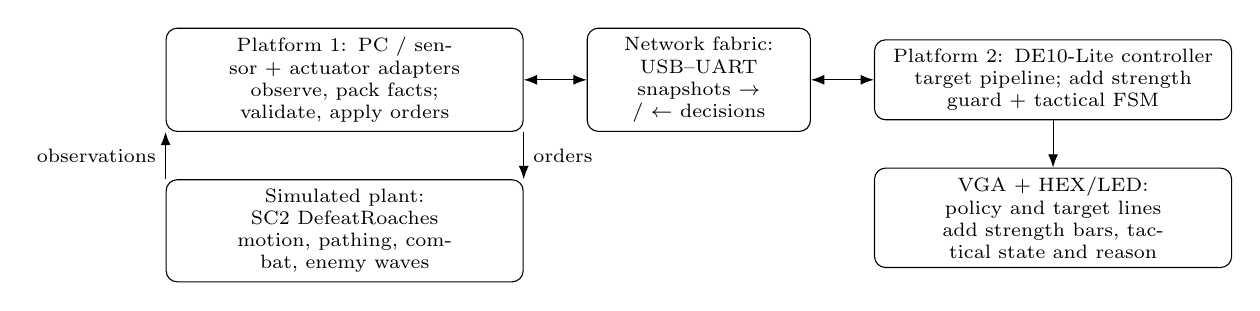
\begin{tikzpicture}[>=Latex,every node/.style={font=\scriptsize,align=center},
box/.style={draw,rounded corners,minimum height=0.65cm},node distance=0.45cm]
\node[box,text width=4.3cm] (host) {Platform 1: PC / sensor + actuator adapters\\observe, pack facts; validate, apply orders};
\node[box,text width=2.6cm,right=0.8cm of host] (net) {Network fabric: USB--UART\\snapshots $\rightarrow$ / $\leftarrow$ decisions};
\node[box,text width=4.3cm,right=0.8cm of net] (fpga) {Platform 2: DE10-Lite controller\\target pipeline; add strength guard + tactical FSM};
\node[box,text width=4.3cm,below=0.6cm of host] (plant) {Simulated plant: SC2 DefeatRoaches\\motion, pathing, combat, enemy waves};
\node[box,text width=4.3cm,below=0.6cm of fpga] (vga) {VGA + HEX/LED: policy and target lines\\add strength bars, tactical state and reason};
\draw[<->] (host) -- (net);
\draw[<->] (net) -- (fpga);
\draw[->] (plant.north west) -- node[left]{observations} (host.south west);
\draw[->] (host.south east) -- node[right]{orders} (plant.north east);
\draw[->] (fpga) -- (vga);
\end{tikzpicture}
\end{center}
\vspace{-6pt}
Adapted from Lee--Seshia Fig.~1.1 [1]. Sensors/actuators are API adapters; SC2 substitutes for a physical plant. The PC transports facts and translates FPGA decisions; SC2 executes movement, firing and damage. Built-in auto-targeting can occur between decisions.

\heading{3. Highest-value algorithms and observable FSM behavior}
\begin{itemize}
\item \textbf{Required foundation: nearest versus weakest-in-range focus fire [2].} Preserve integer ranking, squared distances and deterministic index ties. Show one saved snapshot under both switches, then reset matched live episodes. This controls \emph{who} receives ATTACK orders; a policy toggle is not itself an ATTACK/RETREAT transition.
\item \textbf{Planned extension: Lanchester-inspired strength guard [3].} For homogeneous forces per side, compute $P_F=k_FN_F^2$ and $P_E=k_EN_E^2$, where $k_F\propto\mathrm{DPS}_F/\mathrm{HPmax}_E$ and conversely for $k_E$. Use fixed integer coefficients, a 17-entry square lookup, widened products/comparisons; no ODE solver, division or square root. Add friendly HP and explicit encounter reset. Proposed guard: retreat if $4P_F<3P_E$ or friendly HP is at most 25\% of encounter-initial maximum. Latch RETREAT until reset; HOLD within one map unit of an authored safe point. Otherwise ATTACK when enemies exist; HOLD when none. VGA adds strength bars, state and guard reason. Freeze bounds, coefficients, widths, transition priority and move/hold semantics before HDL. Partial health, range, geometry and waves limit the square-law model. Judge retreat by survival, separately from victory/score.
\item \textbf{Defer:} damage reservations (no gain in the existing software sweep), target hysteresis and cooldown kiting. No mixed armies, learning, search or general navigation.
\end{itemize}

\heading{4. Hardware value, scope and verification}
MAX 10 \texttt{10M50DAF484C7G}, 50\,MHz; custom UART RX/TX (115200, 8-N-1), checksum/parser FSMs, register records, three-stage distance/ranking pipeline, reply FSM and 640$\times$480 VGA using a 25\,MHz pixel enable. No RAM/PLL IP is required by the existing design. PR~\#6 reports 1,216 reference-matching cases in each simulator and board CLOSEST tests, 32\% LEs and +4.283\,ns setup slack. Reported core maximum: 258 clocks (5.16\,$\mu$s); round trip median: 15.9\,ms. These are baseline results, not new measurements or CPU-speedup evidence. Demonstrate concurrent communication/control/display, predictable core cycles, switch-selected decisions and error recovery. Check both policies and new state/guard sequences against an independent reference; refit/timing-check extensions. Use step mode, eight game loops/decision; log versions, seeds, score/outcome, survivors, errors and separate core/link latency. Gate live retreat integration by Nov.~20; if blocked, seek assessed-scope revision and label the strength display advisory.

\heading{5. Realistic ownership and delivery}
\textbf{Lead:} architecture, algorithms/FSM, protocol/SC2 integration, reviews and final sign-off.
\textbf{Development partner:} own board, UART and VGA; independent setup, strength-bar/status display and reference/board regression assistance; lead owns integration.
\textbf{Report partner:} references, architecture explanation, evidence tables and report assembly.
\textbf{Demo partner:} scenario setup, matched-run evidence, cabling/checklist and timed rehearsal/narration.
Names remain unassigned; these are future deliverables, not retrospective equal coding credit. Freeze by Nov.~26; evaluate/rehearse Nov.~27--Dec.~1; demo/report Dec.~2.

\vspace{3pt}
\footnotesize
[1] E. A. Lee and S. A. Seshia, \href{https://ptolemy.berkeley.edu/books/leeseshia/releases/LeeSeshia_DigitalV2_3.pdf}{\emph{Introduction to Embedded Systems}}, 2nd ed., Fig.~1.1, p.~6; Sec.~3.3 (2017).\quad
[2] D. Churchill and M. Buro, \href{https://davechurchill.ca/publications/pdf/combat13.pdf}{\emph{Portfolio Greedy Search and Simulation for Large-Scale Combat in StarCraft}}, Sec.~III (2013).\quad
[3] M. Stanescu, N. Barriga and M. Buro, \href{https://cdn.aaai.org/ojs/12780/12780-52-16297-1-2-20201228.pdf}{\emph{Using Lanchester Attrition Laws for Combat Prediction in StarCraft}}, AIIDE (2015). Our guard is an engineering adaptation, not their learned model.
\end{document}
